\documentclass[UTF8,a4paper,12pt,fontset=none]{ctexart}

\usepackage[a4paper,margin=2.2cm]{geometry}
\usepackage{array}
\usepackage{booktabs}
\usepackage{caption}
\usepackage{enumitem}
\usepackage{float}
\usepackage{fontspec}
\usepackage{graphicx}
\usepackage{hyperref}
\usepackage{listings}
\usepackage{siunitx}
\usepackage{subcaption}
\usepackage{tabularx}
\usepackage{xcolor}

\hypersetup{colorlinks=true,linkcolor=blue!60!black,urlcolor=blue!60!black}
\defaultCJKfontfeatures{AutoFakeSlant=.2}
\setCJKmainfont{Songti SC}
\setCJKsansfont{Heiti SC}
\setCJKmonofont{Heiti SC}
\setmonofont{Menlo}
\setlength{\parindent}{2em}
\setlength{\parskip}{0.35em}
\graphicspath{{../results/figures/}}
\captionsetup{font=small}
\sisetup{round-mode=places,round-precision=3}

\definecolor{AccentA}{HTML}{0B6E4F}
\definecolor{AccentB}{HTML}{1D4E89}
\definecolor{AccentC}{HTML}{F4A259}
\definecolor{AccentD}{HTML}{C73E1D}
\definecolor{CodeBg}{HTML}{F7F7F7}

\lstset{
  basicstyle=\ttfamily\small,
  backgroundcolor=\color{CodeBg},
  frame=single,
  framerule=0pt,
  xleftmargin=1em,
  xrightmargin=1em,
  breaklines=true,
  columns=fullflexible,
  keywordstyle=\color{AccentB}\bfseries,
  commentstyle=\color{AccentA},
  stringstyle=\color{AccentD},
  showstringspaces=false
}

\title{\bfseries 中山大学计算机院本科生实验报告}
\author{}
\date{}

\begin{document}

\begin{titlepage}
  \centering
  {\zihao{2}\bfseries 中山大学计算机院本科生实验报告\par}
  \vspace{0.5em}
  {\zihao{4}（2025学年春季学期）\par}
  \vspace{2em}

  \begin{tabularx}{0.9\textwidth}{>{\bfseries}p{4cm}X}
    课程名称： & 并行程序设计与算法 \\
    实验题目： & Lab2 基于 MPI 的并行矩阵乘法（进阶） \\
    批改人： & \\
    专业（方向）： & \\
    学号： & 23336128 \\
    姓名： & 梁力航 \\
    Email： & \\
    完成日期： & 2026年4月11日 \\
  \end{tabularx}

  \vfill
  \begin{minipage}{0.88\textwidth}
    \small
    本报告围绕 Lab2 的两种 MPI 矩阵乘法实现展开：一版沿用点对点通信作为对照组，另一版使用
    \texttt{MPI\_Type\_create\_struct}、\texttt{MPI\_Scatterv}、\texttt{MPI\_Bcast}、
    \texttt{MPI\_Gatherv} 完成集合通信实现。实验目标不是简单证明“集合通信一定更快”，而是分析不同通信组织方式在不同问题规模和进程数下的真实收益与边界。
  \end{minipage}
\end{titlepage}

\section{实验目的}

本实验在 Lab1 点对点 MPI 矩阵乘法的基础上，继续完成并行矩阵乘法的工程化闭环。具体目标如下：

\begin{enumerate}[leftmargin=2.2em]
  \item 实现点对点对照版 \texttt{mpi\_v1\_p2p}，作为 Lab1 思路在 Lab2 中的延续；
  \item 实现集合通信版 \texttt{mpi\_v2\_collective}，使用 \texttt{MPI\_Scatterv}、\texttt{MPI\_Bcast} 和 \texttt{MPI\_Gatherv} 组织数据流；
  \item 使用 \texttt{MPI\_Type\_create\_struct} 将 \texttt{m/n/k/seed/dump\_matrix} 聚合成统一配置结构并广播；
  \item 在 \texttt{1/2/4/8/16} 个进程、\texttt{128/256/512/1024/2048} 五种规模下完成 benchmark；
  \item 生成运行时间、加速比、并行效率、版本对比和热力图等可视化结果，并形成可直接提交的实验报告。
\end{enumerate}

\section{实验平台与环境}

本实验在 Apple Silicon 本机环境完成，实验环境如下：

\begin{table}[H]
  \centering
  \caption{实验环境信息}
  \renewcommand{\arraystretch}{1.2}
  \begin{tabularx}{0.92\textwidth}{>{\bfseries}p{4cm}X}
    \toprule
    项目 & 配置 \\
    \midrule
    操作系统 & macOS 26.3.1 (Build 25D771280a) \\
    内核与架构 & Darwin 25.3.0, arm64 \\
    MPI 实现 & Open MPI 5.0.9 \\
    C/C++ 编译器 & Apple clang 21.0.0 \\
    CPU & Apple M4 \\
    CPU 核数 & 10 \\
    内存 & 16 GB \\
    运行方式 & \texttt{mpirun --oversubscribe} \\
    Python 工作流 & \texttt{uv run python ...} \\
    \bottomrule
  \end{tabularx}
\end{table}

这里需要特别说明两点。第一，实验环境只有 10 个 CPU 核心，但测试维度包含 16 个 MPI 进程，因此高进程数组合一定带有 oversubscribe 的现实影响。第二，本实验的 Python 工具链统一在 \texttt{lab/lab2} 目录中通过 \texttt{uv} 执行，以保证 benchmark、绘图和导表依赖来自同一环境。

\section{实验过程与核心实现}

\subsection{总体实现思路}

Lab2 沿用 Lab1 的按行划分思想，但将代码组织扩展为两个版本：

\begin{enumerate}[leftmargin=2.2em]
  \item \textbf{点对点版本}：rank 0 生成矩阵，显式使用 \texttt{MPI\_Send}/\texttt{MPI\_Recv} 分发矩阵 A 的行块和完整矩阵 B，再回收结果矩阵 C；
  \item \textbf{集合通信版本}：rank 0 先广播统一配置，再使用 \texttt{MPI\_Scatterv} 分发 A、\texttt{MPI\_Bcast} 广播 B、\texttt{MPI\_Gatherv} 汇总 C；
  \item \textbf{统一输出契约}：两个版本均输出稳定的 \texttt{key=value} 字段，供 benchmark 脚本解析；
  \item \textbf{统一随机矩阵生成}：固定使用种子 \texttt{20250401}，保证不同进程数、不同实现之间的 checksum 可比。
\end{enumerate}

\subsection{点对点版本 \texttt{mpi\_v1\_p2p}}

\texttt{mpi\_v1\_p2p} 的数据流与 Lab1 一致：rank 0 首先生成完整矩阵，然后按行数将矩阵 A 的子块逐个发送给其他进程，并将矩阵 B 完整发送到所有进程。各进程独立完成本地矩阵乘法后，再通过点对点通信将 C 的局部结果交回 rank 0 汇总。这个实现的优点是流程直观、易于验证，缺点是根进程承担了明显的调度和收发压力。

\subsection{集合通信版本 \texttt{mpi\_v2\_collective}}

\texttt{mpi\_v2\_collective} 并不是简单把点对点调用换一批 API 名字，而是把通信组织方式改成了“配置广播 + 数据分发 + 结果回收”的集合通信流水线。具体做法是：

\begin{enumerate}[leftmargin=2.2em]
  \item rank 0 解析命令行参数，构造 \texttt{MatrixRunConfig}；
  \item 通过 \texttt{MPI\_Type\_create\_struct} 建立配置结构体对应的 MPI datatype；
  \item 将配置结构体一次性广播到所有进程；
  \item 各进程据此独立计算行划分数组 \texttt{row\_counts} 与 \texttt{row\_displs}；
  \item rank 0 生成矩阵 A、B；
  \item 使用 \texttt{MPI\_Scatterv} 分发 A 的行块，使用 \texttt{MPI\_Bcast} 广播完整 B；
  \item 各进程完成本地计算后，使用 \texttt{MPI\_Gatherv} 回收 C。
\end{enumerate}

这个版本的工程意义在于：通信组织更集中、控制流更清晰，也为后续继续演化第三版优化实现保留了更干净的边界。

\subsection{结构化配置通信的设计理由}

如果仍然像初学版程序那样逐字段广播 \texttt{m}、\texttt{n}、\texttt{k}、\texttt{seed} 和 \texttt{dump\_matrix}，代码会快速变得零散，也不利于后续扩展新配置字段。将这些参数收敛到 \texttt{MatrixRunConfig} 中，再通过 \texttt{MPI\_Type\_create\_struct} 建立 datatype，有两个直接收益：

\begin{itemize}
  \item 一次广播即可同步完整运行配置，避免顺序错误和重复代码；
  \item 后续新增字段时，只需要维护结构体和 datatype 构造逻辑，不需要重写通信协议。
\end{itemize}

\subsection{核心代码片段}

\subsubsection{行划分逻辑}

\begin{lstlisting}[language=C++]
inline void compute_row_partition(int m, int size,
                                  std::vector<int>& row_counts,
                                  std::vector<int>& row_displs) {
    row_counts.assign(size, 0);
    row_displs.assign(size, 0);
    const int base = m / size;
    const int remainder = m % size;
    for (int p = 0; p < size; ++p) {
        row_counts[p] = base + (p < remainder ? 1 : 0);
        row_displs[p] = (p == 0) ? 0 : row_displs[p - 1] + row_counts[p - 1];
    }
}
\end{lstlisting}

这段逻辑决定每个进程负责的行数，并处理矩阵行数不能被进程数整除的情况。它是两个版本共享的公共基础。

\subsubsection{\texttt{MPI\_Type\_create\_struct} 配置广播}

\begin{lstlisting}[language=C++]
inline MPI_Datatype build_config_type() {
    MatrixRunConfig sample{};
    int block_lengths[5] = {1, 1, 1, 1, 1};
    MPI_Aint displacements[5];
    MPI_Datatype types[5] = {
        MPI_INT, MPI_INT, MPI_INT, MPI_UINT64_T, MPI_INT
    };

    MPI_Aint base_address;
    MPI_Get_address(&sample, &base_address);
    MPI_Get_address(&sample.m, &displacements[0]);
    MPI_Get_address(&sample.n, &displacements[1]);
    MPI_Get_address(&sample.k, &displacements[2]);
    MPI_Get_address(&sample.seed, &displacements[3]);
    MPI_Get_address(&sample.dump_matrix, &displacements[4]);

    for (MPI_Aint& displacement : displacements) {
        displacement -= base_address;
    }

    MPI_Datatype config_type;
    MPI_Type_create_struct(5, block_lengths, displacements, types, &config_type);
    MPI_Type_commit(&config_type);
    return config_type;
}
\end{lstlisting}

这段代码把结构体字段映射到 MPI datatype 中，使配置广播从“多个标量消息”收敛为“一次结构化广播”。

\subsubsection{集合通信主路径}

\begin{lstlisting}[language=C++]
MPI_Bcast(&config, 1, config_type, 0, MPI_COMM_WORLD);
MPI_Scatterv(rank == 0 ? a.data() : nullptr,
             a_counts.data(), a_displs.data(), MPI_DOUBLE,
             local_a.data(), a_counts[rank], MPI_DOUBLE,
             0, MPI_COMM_WORLD);
MPI_Bcast(b.data(), config.n * config.k, MPI_DOUBLE, 0, MPI_COMM_WORLD);

local_matmul(local_a.data(), b.data(), local_c.data(),
             row_counts[rank], config.n, config.k);

MPI_Gatherv(local_c.data(), c_counts[rank], MPI_DOUBLE,
            rank == 0 ? c.data() : nullptr,
            c_counts.data(), c_displs.data(), MPI_DOUBLE,
            0, MPI_COMM_WORLD);
\end{lstlisting}

这段路径体现了 \texttt{mpi\_v2\_collective} 的核心：配置、输入分发和结果回收都放在更标准的 MPI 集合通信接口上完成。

\section{Benchmark 设计与正确性校验}

本实验使用如下 benchmark 维度：

\begin{itemize}
  \item 版本：\texttt{mpi\_v1\_p2p}、\texttt{mpi\_v2\_collective}
  \item 进程数：1、2、4、8、16
  \item 矩阵规模：128、256、512、1024、2048
  \item 每组重复次数：3
  \item 固定随机种子：20250401
\end{itemize}

benchmark 脚本除了记录平均时间外，还检查如下信号：

\begin{enumerate}[leftmargin=2.2em]
  \item 程序返回码是否为 0；
  \item 标准输出是否包含完整的 \texttt{key=value} 字段；
  \item 同一配置重复运行时 checksum 是否一致；
  \item 多进程结果与单进程基线 checksum 是否一致。
\end{enumerate}

本次正式全量 benchmark 共生成 50 组配置记录，结果状态全部为 \texttt{ok}。这意味着在当前测试范围内，两套实现都完成了正确性校验，没有出现字段缺失、运行失败或 checksum 不一致问题。

\section{实验结果与可视化分析}

\subsection{精简运行时间表}

为了避免把全部 50 组原始结果直接堆入正文，表 \ref{tab:compact-runtime} 只保留三个关键规模（512、1024、2048）和三个代表性进程数（1、4、16），用于展示总体趋势。

\begin{table}[H]
  \centering
  \caption{关键规模与关键进程数下的平均运行时间（秒）}
  \label{tab:compact-runtime}
  \small
  \renewcommand{\arraystretch}{1.2}
  \begin{tabularx}{\textwidth}{
    >{\centering\arraybackslash}m{2.3cm}
    >{\centering\arraybackslash}m{1.4cm}
    >{\centering\arraybackslash}X
    >{\centering\arraybackslash}X
    >{\centering\arraybackslash}X
  }
    \toprule
    版本 & 进程数 & 512 & 1024 & 2048 \\
    \midrule
    \texttt{mpi\_v1\_p2p} & 1  & 0.123033 & 0.997698 & 23.445053 \\
    \texttt{mpi\_v1\_p2p} & 4  & 0.048867 & 1.121589 & 15.619476 \\
    \texttt{mpi\_v1\_p2p} & 16 & 0.057792 & 1.112545 & 12.829863 \\
    \texttt{mpi\_v2\_collective} & 1  & 0.121091 & 0.953602 & 21.418602 \\
    \texttt{mpi\_v2\_collective} & 4  & 0.051294 & 0.694170 & 15.334143 \\
    \texttt{mpi\_v2\_collective} & 16 & 0.084111 & 0.968709 & 10.901446 \\
    \bottomrule
  \end{tabularx}
\end{table}

\subsection{最佳配置与最佳加速比摘要}

表 \ref{tab:best-config} 汇总了每个版本在不同规模下的最佳时间配置，以及对应的最佳加速比。这里的“最佳时间配置”和“最佳加速比配置”在本实验中恰好一致，因此可以直接反映不同规模下的并行甜点区间。

\begin{table}[H]
  \centering
  \caption{各版本在不同规模下的最佳配置摘要}
  \label{tab:best-config}
  \small
  \renewcommand{\arraystretch}{1.2}
  \begin{tabularx}{\textwidth}{
    >{\centering\arraybackslash}m{2.5cm}
    >{\centering\arraybackslash}m{1.2cm}
    >{\centering\arraybackslash}m{1.6cm}
    >{\centering\arraybackslash}X
    >{\centering\arraybackslash}X
  }
    \toprule
    版本 & 规模 & 最优进程数 & 最优时间（秒） & 最佳加速比 \\
    \midrule
    \texttt{mpi\_v1\_p2p} & 128  & 1  & 0.001177 & 1.000 \\
    \texttt{mpi\_v1\_p2p} & 256  & 4  & 0.005527 & 2.042 \\
    \texttt{mpi\_v1\_p2p} & 512  & 4  & 0.048867 & 2.518 \\
    \texttt{mpi\_v1\_p2p} & 1024 & 2  & 0.609451 & 1.637 \\
    \texttt{mpi\_v1\_p2p} & 2048 & 16 & 12.829863 & 1.827 \\
    \midrule
    \texttt{mpi\_v2\_collective} & 128  & 1  & 0.001708 & 1.000 \\
    \texttt{mpi\_v2\_collective} & 256  & 2  & 0.006185 & 2.169 \\
    \texttt{mpi\_v2\_collective} & 512  & 4  & 0.051294 & 2.361 \\
    \texttt{mpi\_v2\_collective} & 1024 & 2  & 0.636073 & 1.499 \\
    \texttt{mpi\_v2\_collective} & 2048 & 16 & 10.901446 & 1.965 \\
    \bottomrule
  \end{tabularx}
\end{table}

\subsection{运行时间与版本对比}

\begin{figure}[H]
  \centering
  \begin{subfigure}[t]{0.48\textwidth}
    \centering
    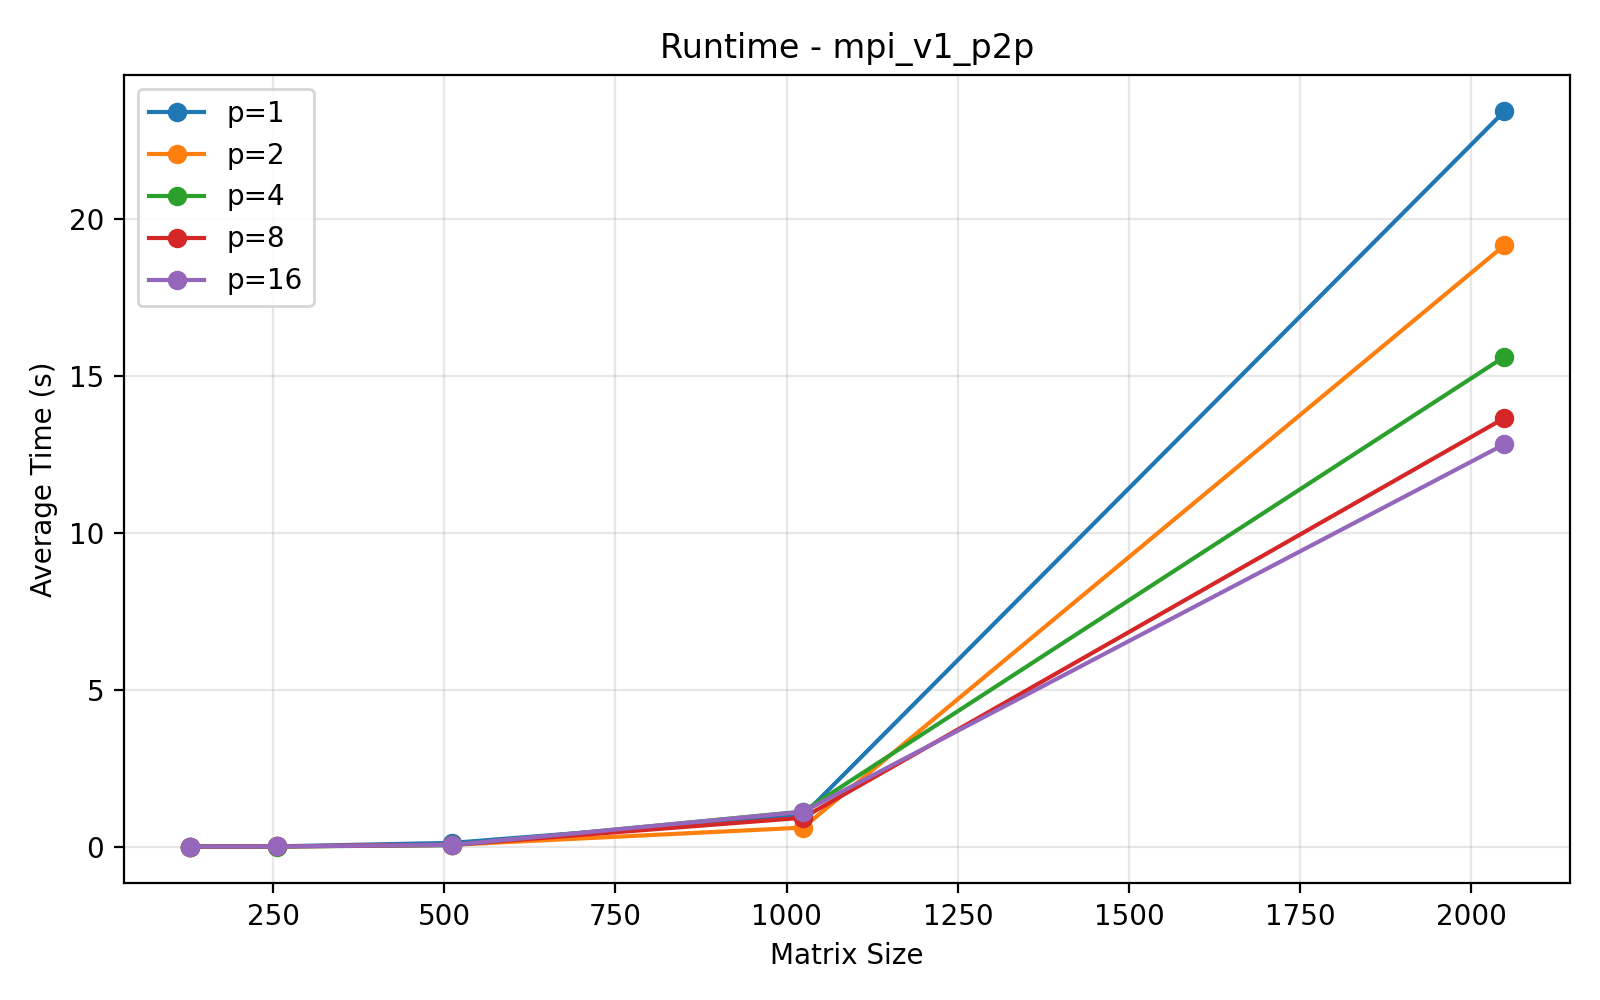
\includegraphics[width=\textwidth]{runtime_mpi_v1_p2p.png}
    \caption{\texttt{mpi\_v1\_p2p} 运行时间}
  \end{subfigure}
  \hfill
  \begin{subfigure}[t]{0.48\textwidth}
    \centering
    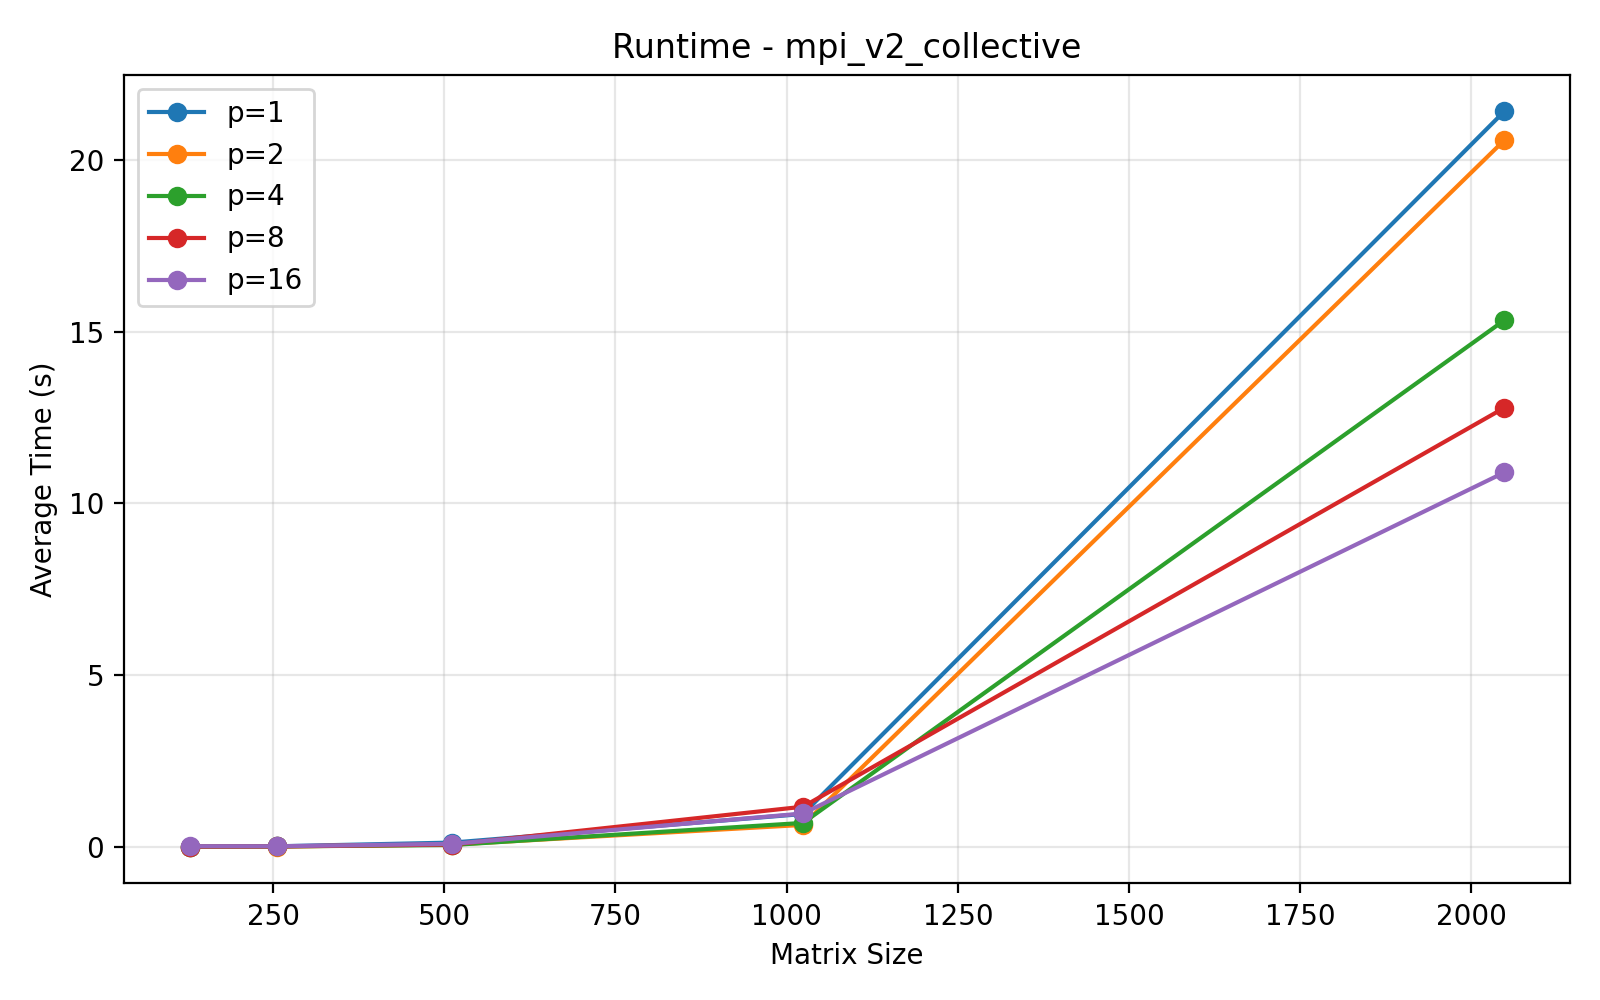
\includegraphics[width=\textwidth]{runtime_mpi_v2_collective.png}
    \caption{\texttt{mpi\_v2\_collective} 运行时间}
  \end{subfigure}

  \vspace{0.8em}

  \begin{subfigure}[t]{0.68\textwidth}
    \centering
    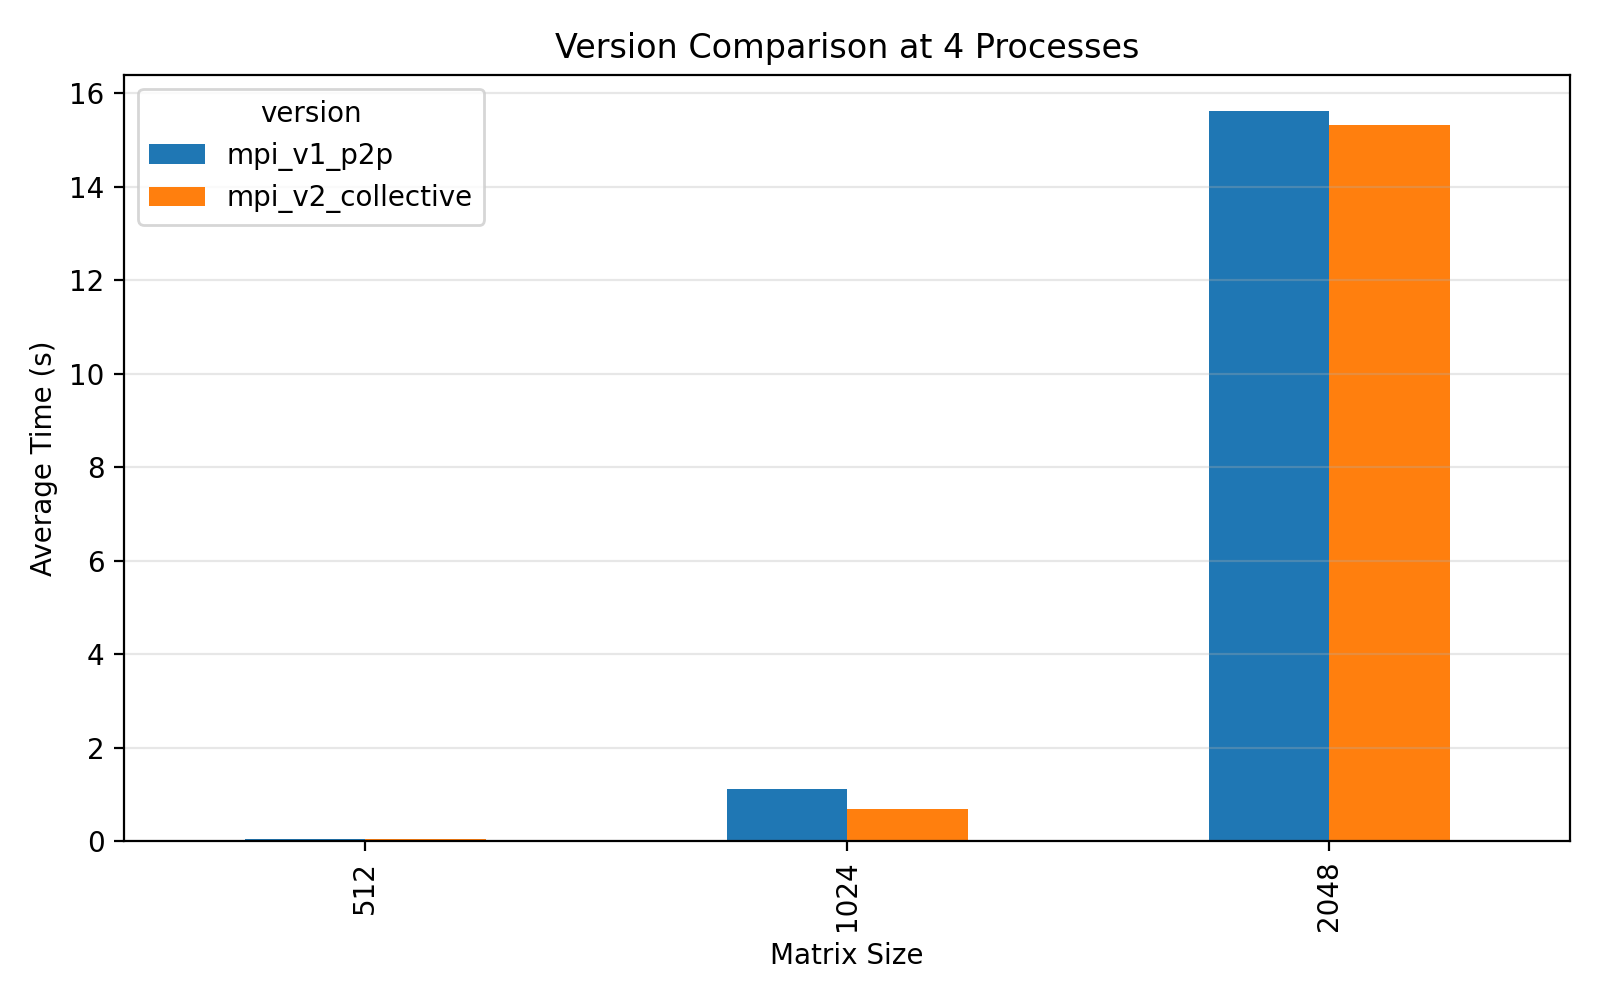
\includegraphics[width=\textwidth]{version_comparison.png}
    \caption{关键规模下的版本对比}
  \end{subfigure}
  \caption{运行时间与版本对比可视化}
  \label{fig:runtime-and-version}
\end{figure}

从图 \ref{fig:runtime-and-version} 和表 \ref{tab:compact-runtime} 可以先得出一个直接判断：本实验的主要收益来自中大规模下的计算分摊，而不是通信模式名称本身。128 规模下，两版本最优时间都出现在单进程，说明问题规模太小，通信和进程管理开销会吃掉并行收益。进入 256 和 512 规模后，2 到 4 个进程开始显著获益，说明此时计算量已经足以覆盖一部分通信成本。到 2048 规模时，两版本的最优时间都出现在 16 进程，但由于机器只有 10 核，这里的收益已经明显受到 oversubscribe 和带宽竞争限制，速度提升远低于线性理想值。

版本对比也体现出一个更有价值的事实：\texttt{mpi\_v2\_collective} 并不是在所有场景下都更快。以 512 规模为例，4、8、16 进程下反而是点对点版本略快；但到了 1024 规模的 4 进程和 2048 规模的 8、16 进程，集合通信版本开始明显占优。经验上，这说明集合通信带来的收益更容易在“数据量足够大、根进程调度压力足够明显”的区间体现出来，而在中小规模或较低并行度下，集合通信自身的调度成本并不会自动消失。

\subsection{加速比与并行效率}

\begin{figure}[H]
  \centering
  \begin{subfigure}[t]{0.48\textwidth}
    \centering
    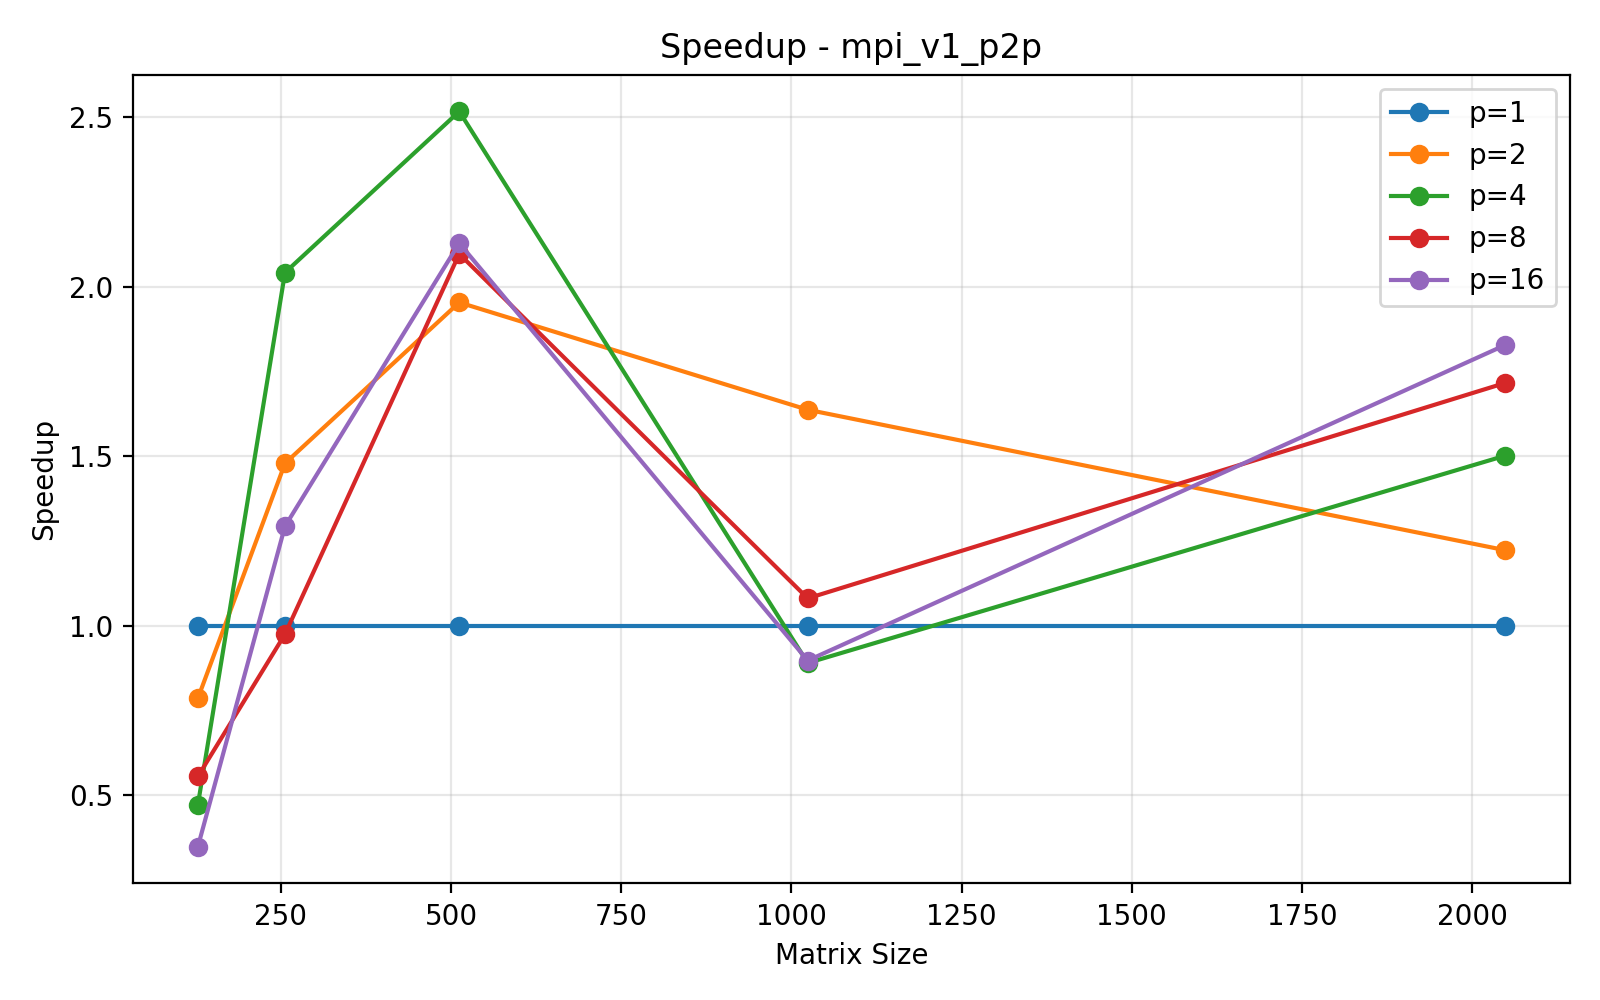
\includegraphics[width=\textwidth]{speedup_mpi_v1_p2p.png}
    \caption{\texttt{mpi\_v1\_p2p} 加速比}
  \end{subfigure}
  \hfill
  \begin{subfigure}[t]{0.48\textwidth}
    \centering
    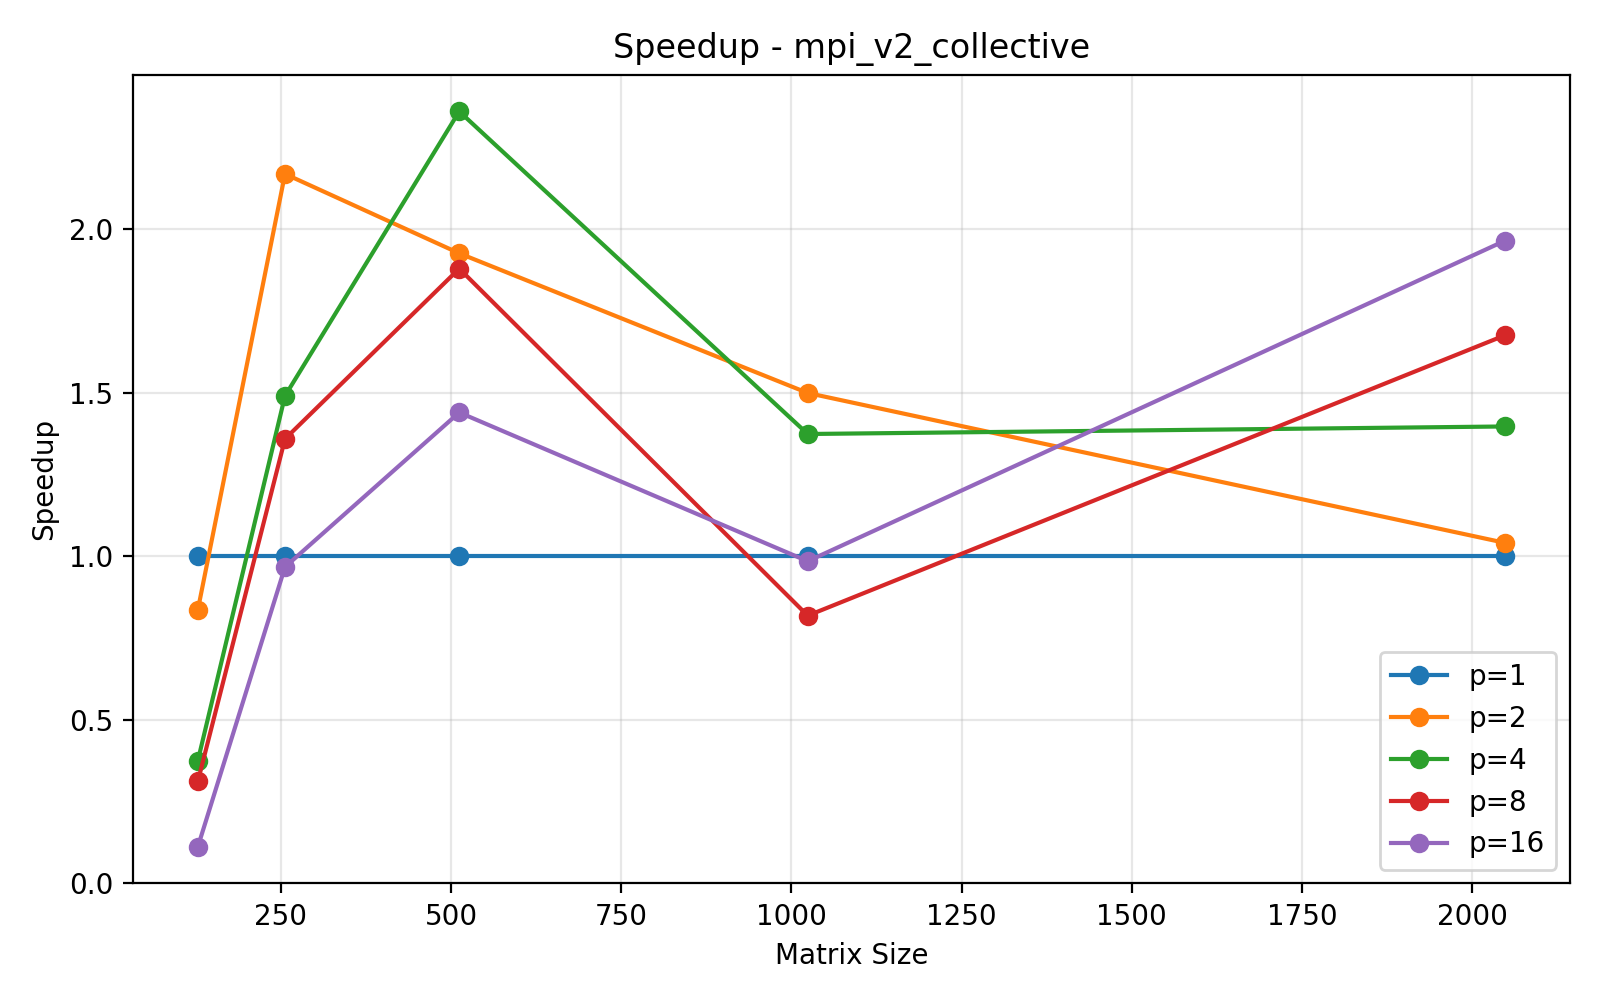
\includegraphics[width=\textwidth]{speedup_mpi_v2_collective.png}
    \caption{\texttt{mpi\_v2\_collective} 加速比}
  \end{subfigure}

  \vspace{0.8em}

  \begin{subfigure}[t]{0.48\textwidth}
    \centering
    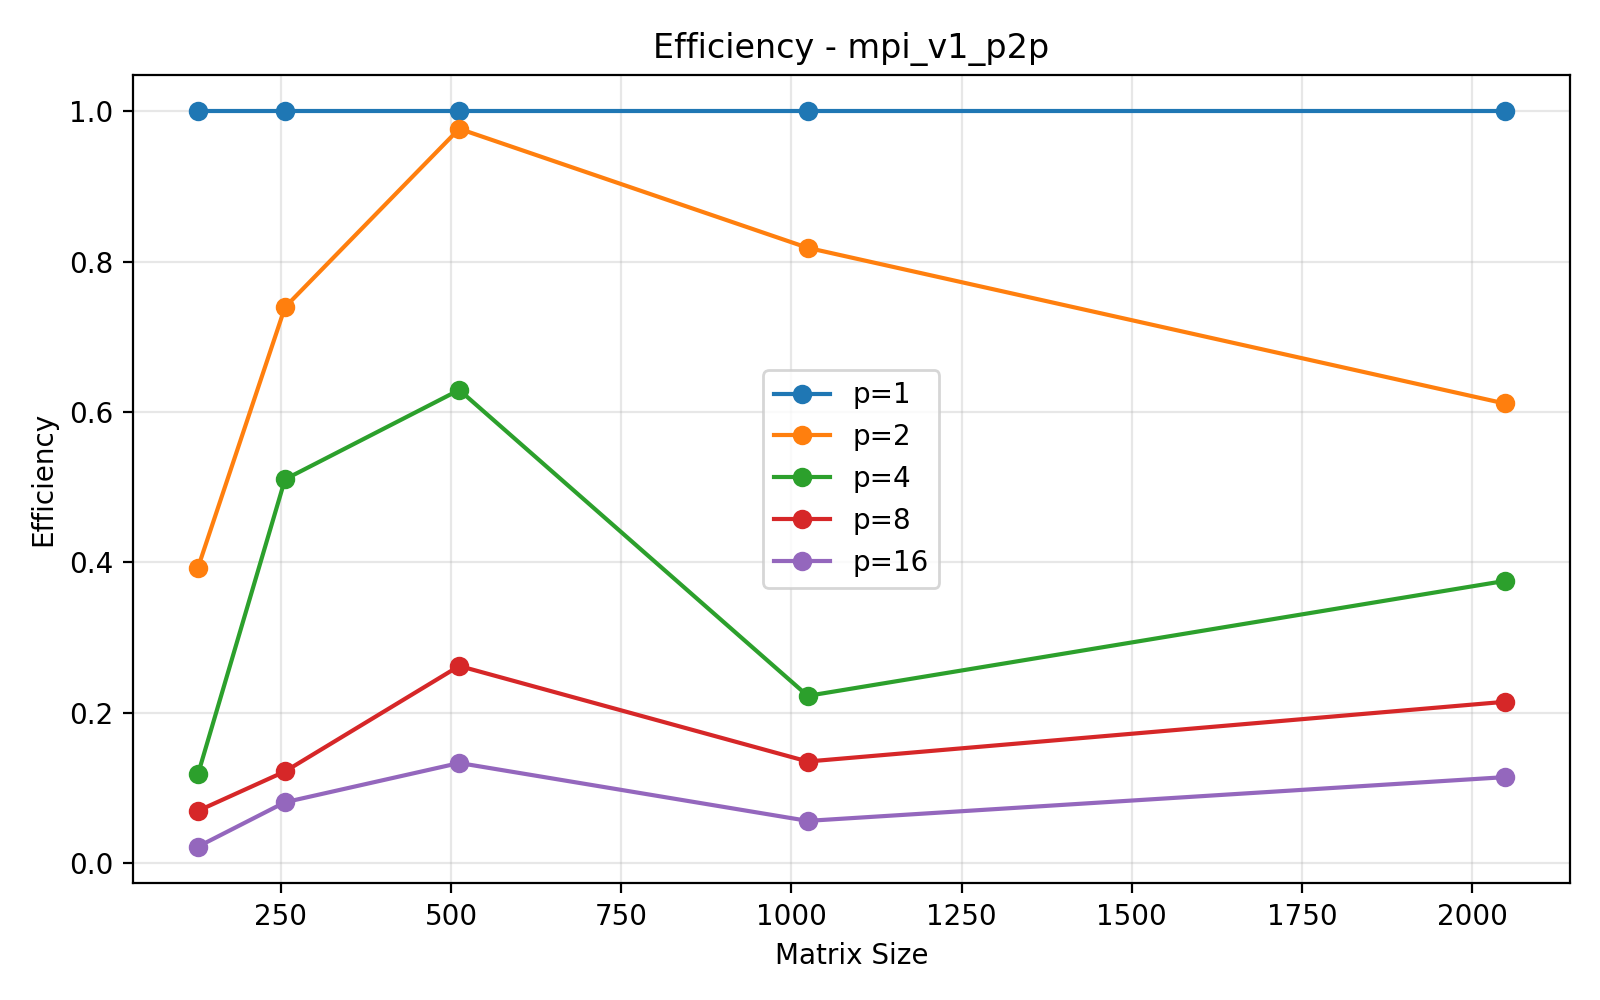
\includegraphics[width=\textwidth]{efficiency_mpi_v1_p2p.png}
    \caption{\texttt{mpi\_v1\_p2p} 并行效率}
  \end{subfigure}
  \hfill
  \begin{subfigure}[t]{0.48\textwidth}
    \centering
    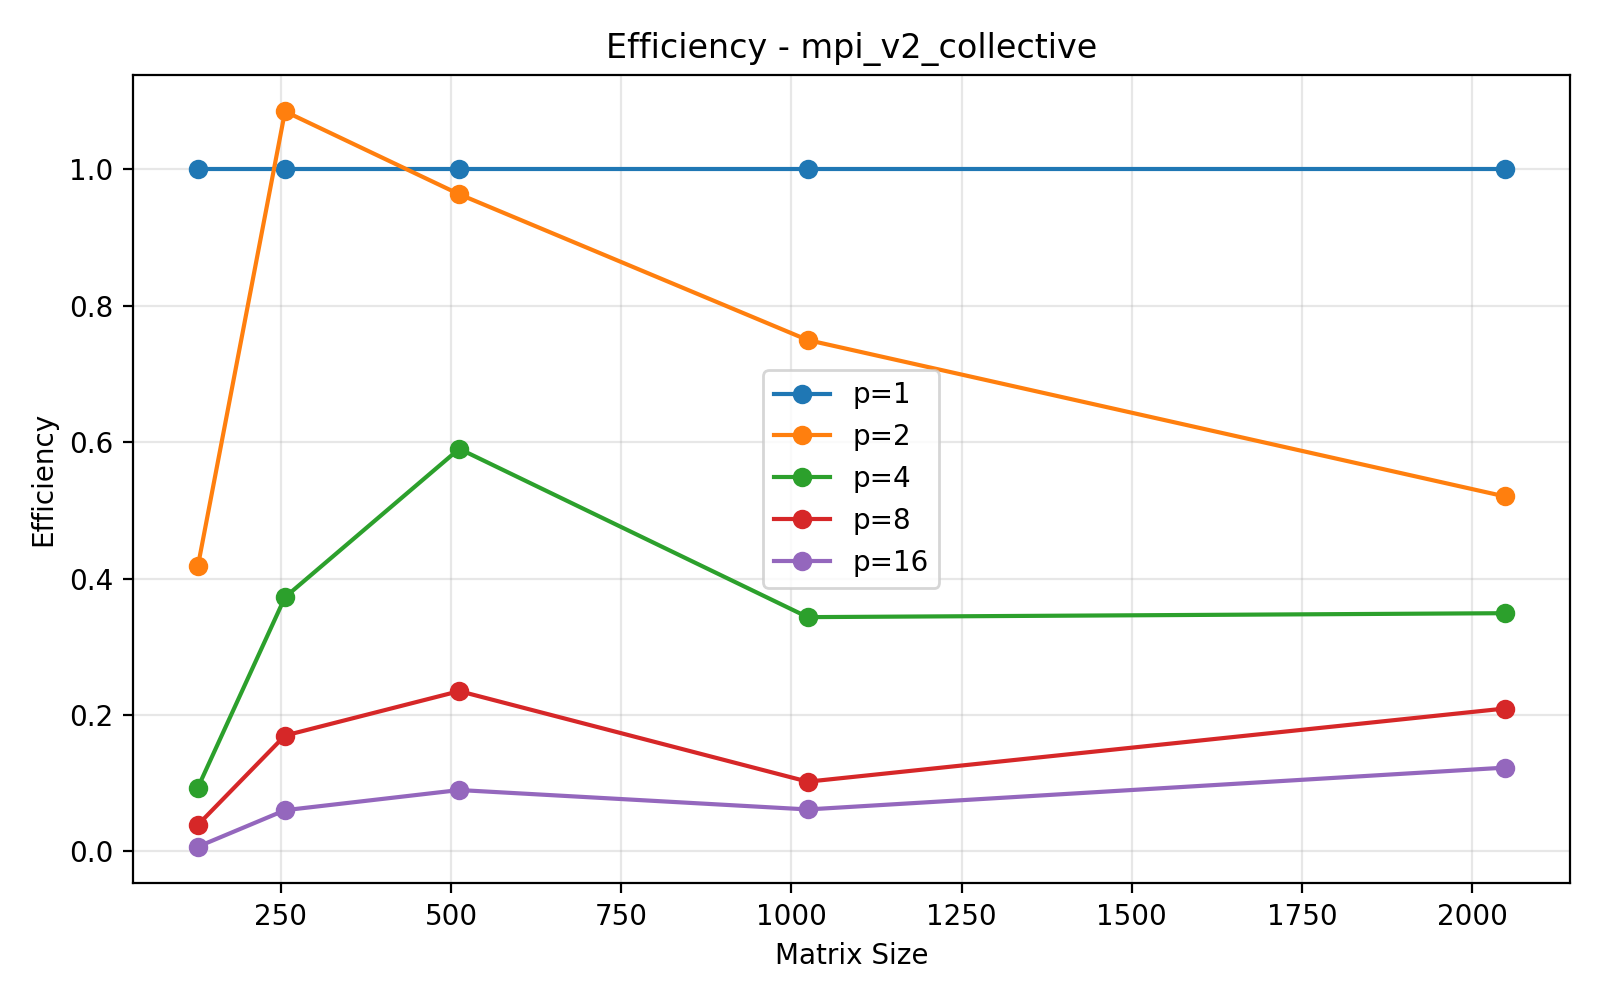
\includegraphics[width=\textwidth]{efficiency_mpi_v2_collective.png}
    \caption{\texttt{mpi\_v2\_collective} 并行效率}
  \end{subfigure}
  \caption{加速比与并行效率可视化}
  \label{fig:speedup-efficiency}
\end{figure}

图 \ref{fig:speedup-efficiency} 说明了并行收益的“甜点区间”。已确认的是，两版本在 256--512 规模、2--4 进程附近最容易得到像样的加速比。例如 \texttt{mpi\_v1\_p2p} 在 512 规模下的最佳加速比为 2.518（4 进程），\texttt{mpi\_v2\_collective} 在 256 规模下的最佳加速比为 2.169（2 进程），在 512 规模下为 2.361（4 进程）。这些结果说明，当问题规模刚好足以抵消通信开销、而进程数又没有高到把同步成本放大时，并行收益最稳定。

从这些信号来看，真正主导结果的张力是“计算分摊收益”和“通信/同步成本”之间的平衡，而不是某种 API 的名义先进性。一个非常实用的观察是：当进程数继续提升到 8 或 16 时，效率曲线会迅速下降。以 2048 规模为例，\texttt{mpi\_v1\_p2p} 在 16 进程下效率仅为 0.114，\texttt{mpi\_v2\_collective} 也只有 0.123。也就是说，大规模虽然还能继续提速，但新增进程并没有按比例转化为收益，说明根因已经从“算得不够快”转向“通信、调度和内存带宽共同限速”。

\subsection{双版本热力图}

\begin{figure}[H]
  \centering
  \begin{subfigure}[t]{0.48\textwidth}
    \centering
    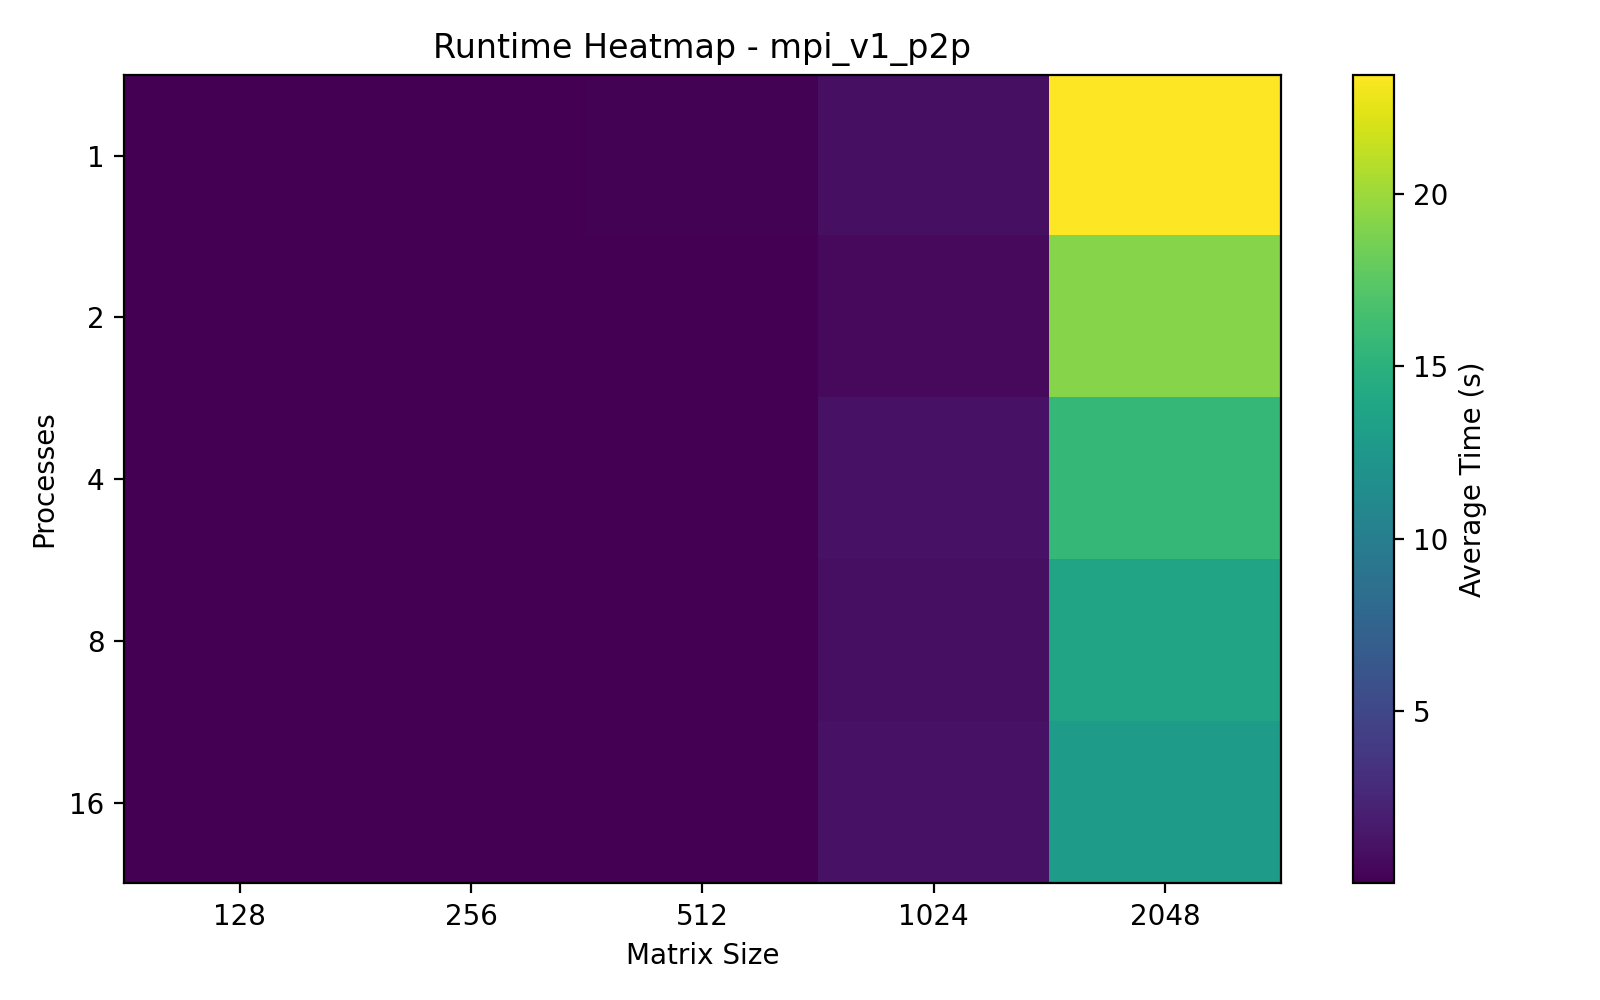
\includegraphics[width=\textwidth]{heatmap_mpi_v1_p2p.png}
    \caption{\texttt{mpi\_v1\_p2p} 热力图}
  \end{subfigure}
  \hfill
  \begin{subfigure}[t]{0.48\textwidth}
    \centering
    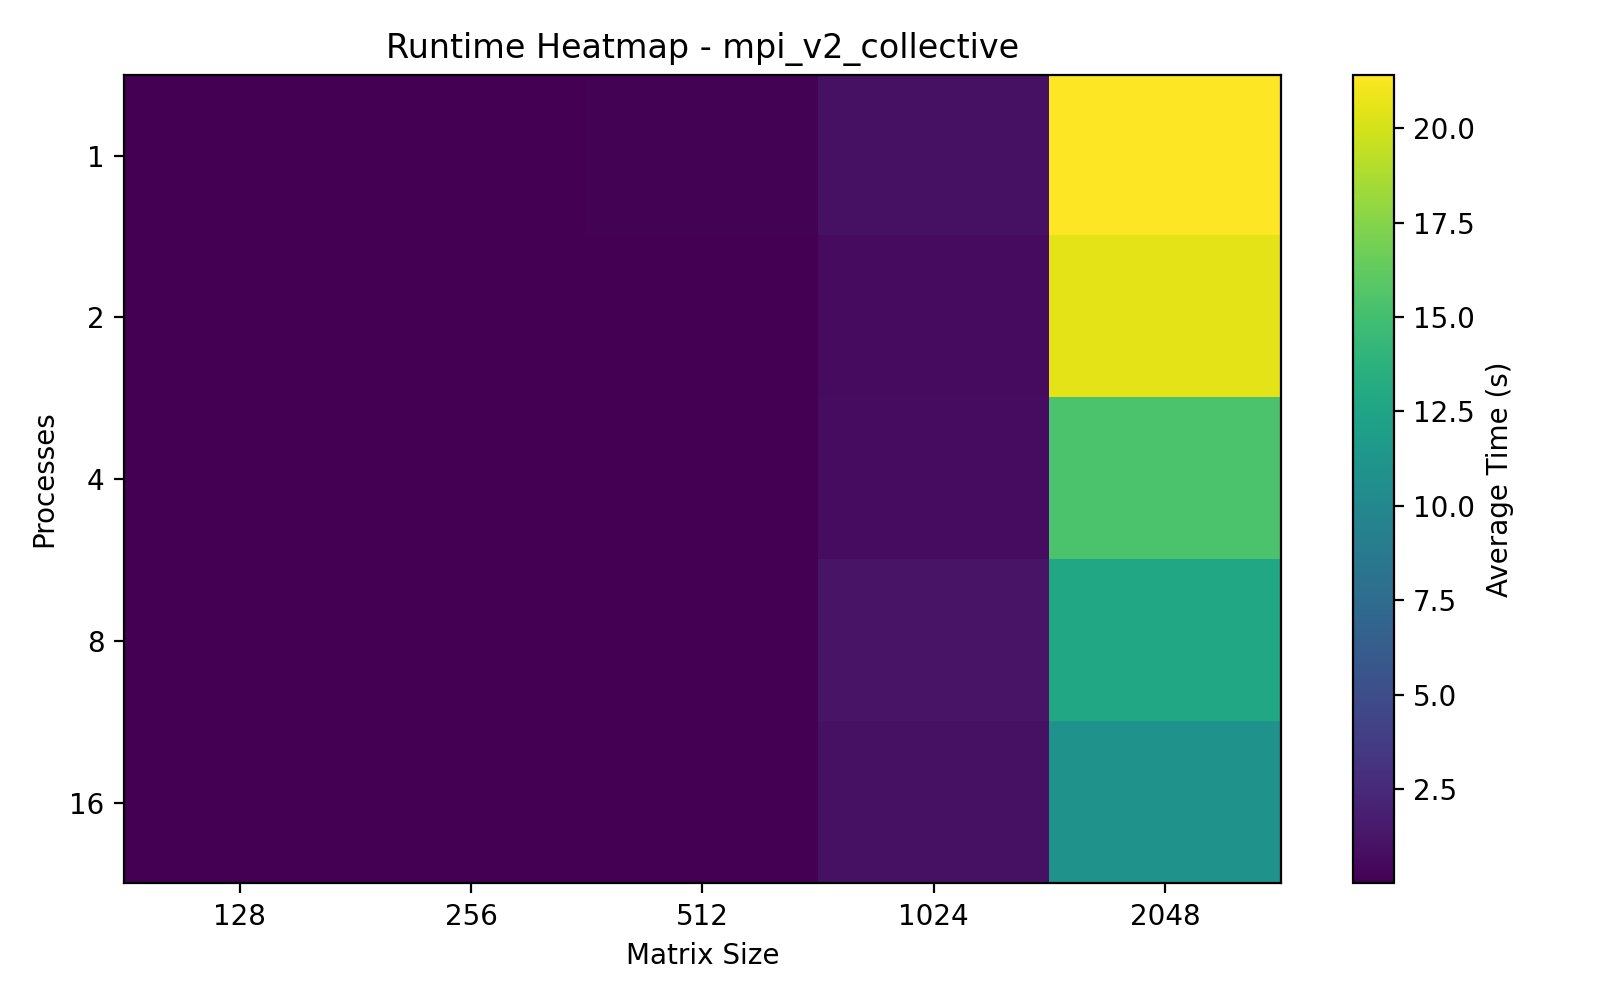
\includegraphics[width=\textwidth]{heatmap_mpi_v2_collective.png}
    \caption{\texttt{mpi\_v2\_collective} 热力图}
  \end{subfigure}
  \caption{双版本运行时间热力图}
  \label{fig:heatmaps}
\end{figure}

热力图让另一个实践信号变得更直观：性能并不是随进程数单调变好，而是存在明显的“平台期”和“回落区”。一个典型例子是 1024 规模。点对点版本在 2 进程时最佳，但到 4 进程反而变慢；集合通信版本在 4 进程上却显著优于点对点版本。这说明进程数变化带来的影响并不只来自“更多并行度”，还来自通信路径组织、rank 0 压力分布以及缓存/带宽行为。

一个可能的情况是：在 1024 和 2048 这种规模下，矩阵 B 的完整广播和矩阵 C 的回收已经足以放大实现细节差异。点对点版本需要 rank 0 显式维护更多发送和接收动作，而集合通信版本把这部分调度交给 MPI 运行时；当进程数提升、消息数量增多时，这种差异会更明显地反映到时间曲线中。不过这并不意味着集合通信永远更好，因为在进程数较少或者规模仍不够大时，collective 的组织开销也可能抵消掉优势。

\section{性能分析}

本实验最重要的判断是：并行矩阵乘法的主要收益来自中大规模下的计算分摊，而不是通信模式名义上的先进性；集合通信的价值更多体现在大规模和较高并行度下对根进程压力的缓解，而不是全程无条件更快。

已经确认的是，小规模问题几乎不适合强行并行化。128 规模下，两版本单进程都是最优；256 和 512 规模开始出现稳定收益，但最优区间仍集中在 2 到 4 个进程附近。说明在这个阶段，计算量刚刚足以覆盖通信成本，多开进程并不一定更划算。

从这些信号来看，root 压力、oversubscribe 和内存带宽是三个最关键的现实因素。点对点版本的问题在于 rank 0 需要显式完成更多数据分发和回收动作；集合通信版本的问题在于 collective 本身也有调度成本，不会免费消失。与此同时，实验机器只有 10 核，但 benchmark 包含 16 进程组合，因此高进程数组合天然带有额外的上下文切换和调度竞争成本。再加上矩阵 B 的完整广播和矩阵 C 的集中回收都会消耗内存带宽，因此效率下降是预期内而不是偶然异常。

一个可能的情况是，1024 规模下的非单调现象反映了实现细节与系统噪声的叠加影响。例如 \texttt{mpi\_v1\_p2p} 在 2 进程时优于 4 进程，而 \texttt{mpi\_v2\_collective} 在 4 进程时又明显优于 \texttt{mpi\_v1\_p2p}。这类现象往往意味着程序已经不再是单纯的算术密集任务，而是开始受制于通信组织方式、消息批次、同步位置以及缓存行为。换句话说，问题已经从“CPU 算得够不够快”转向“系统整体如何搬数据”。

边界与取舍也必须说清楚。本实验比较的是当前两套实现，而不是比较“点对点思想”和“集合通信思想”的绝对优劣。若底层 MPI 实现、机器核心数、消息大小或矩阵存储策略变化，结果也会跟着变。因此，正确的结论不是“以后都应该无脑换成 collective”，而是：当规模足够大、根进程调度压力已经成为瓶颈时，collective 版本更值得优先尝试。

\section{总结}

本实验得到三个比较稳定的结论：

\begin{enumerate}[leftmargin=2.2em]
  \item \textbf{集合通信的工程价值}：\texttt{mpi\_v2\_collective} 的主要价值不在于每个规模都更快，而在于它把配置广播、A 分发和 C 汇总组织得更规范，在 1024 以上规模、4 进程及以上时更容易体现出优势；
  \item \textbf{当前最可能的性能瓶颈}：并不是局部乘法核本身，而是数据搬运、根进程压力、oversubscribe 调度和内存带宽共同作用的结果；
  \item \textbf{后续优化优先方向}：如果继续做 Lab3 或扩展版，最值得优先尝试的是转置矩阵 B 改善局部访存、减少根进程集中式收发压力，以及探索分块矩阵乘法或通信计算重叠，而不是继续简单堆高进程数。
\end{enumerate}

总体来看，Lab2 的结果符合并行程序设计中的一个常见现实：真正决定性能的，不是接口名字有多高级，而是问题规模、数据流组织方式和硬件边界是否匹配。

\end{document}
